\documentclass[10pt,twocolumn]{article}

\usepackage[margin=0.75in]{geometry}
\usepackage{amsmath,amssymb}
\usepackage{graphicx}
\usepackage{booktabs}
\usepackage{hyperref}
\usepackage{natbib}
\usepackage{caption}
\usepackage{xcolor}

\title{Look-Ahead Bias in a Causal Portfolio Backtest: A Corrected \\ Evaluation Protocol and a Null Result}

\author{
  [Author name withheld in draft] \\
  \small Independent Research \\
  \small \texttt{[email withheld]}
}

\date{}

\begin{document}
\maketitle

\begin{abstract}
We present a portfolio construction system that combines causal discovery
(Granger causality and the PC algorithm), double machine learning (DML)
treatment-effect estimation, hidden Markov regime detection, and an
ARIMA/GARCH/LSTM/GBM forecasting ensemble with a causally-adjusted
Markowitz mean-variance optimizer. Using 11 U.S. sector ETFs and seven
macroeconomic treatment variables over a 2010--2026 sample, we walk-forward
backtest the system out-of-sample from May 2021 to January 2024. We report
two results, one methodological and one empirical, and treat the
methodological one as a first-class contribution rather than a footnote.
First, we identify and correct a look-ahead bias in our own initial
evaluation: the treatment-effect model that generates the causal
adjustment was fit once on a data split that overlapped the walk-forward
test window, rather than being re-estimated at each fold's training
cutoff. Correcting this reverses our headline empirical finding. Second,
once corrected, the causally-adjusted portfolio does not improve on
standard mean-variance optimization in this sample (Sharpe ratio
$-0.143$ vs.\ $-0.119$ for plain Markowitz), and neither approach
significantly outperforms a passive S\&P 500 benchmark (Sharpe $+0.093$)
or naive equal weighting (Sharpe $+0.099$); none of the pairwise
differences are statistically significant ($p > 0.25$ for all paired
tests). This is despite the underlying treatment-effect estimates
themselves being far from noise: of all 77 macro-sector pairs tested (7
treatments $\times$ 11 sectors), 27 are significant at an uncorrected
$\alpha=0.05$, and 18 survive Benjamini--Hochberg false-discovery-rate
correction. The disconnect between a substantial fraction of
statistically real treatment effects and a portfolio-level result that
shows no benefit is itself part of the paper's finding (Section
\ref{sec:limitations}): individual effects that are real and precisely
estimated are still too small in magnitude, relative to the base
optimizer's own sensitivity to estimation error, to move a
20\%-capped mean-variance allocation. We argue that the
methodology and the negative result are both worth reporting: the
look-ahead-corrected evaluation protocol is reusable, and the finding
that a correctly-specified causal signal does not measurably help in a
2.7-year, quarterly-rebalanced backtest is informative about the
practical difficulty of using causal inference for tactical asset
allocation at this data scale.
\end{abstract}

\section{Introduction}

Portfolio construction has relied on mean-variance optimization since
\citet{markowitz1952portfolio}, and on correlational and purely
predictive machine learning models more recently
\citep{gu2020empirical}. Both approaches share a limitation: they
characterize statistical association between economic conditions and
asset returns without distinguishing a causal driver from a coincidental
correlate. A sector's return may correlate with an interest-rate move
because rates cause a change in the sector's discount rate and growth
outlook, or because both are driven by a third factor (e.g., aggregate
demand). Only the former licenses the inference "if rates move, this
sector's expected return moves" that a forward-looking allocation
decision actually needs.

This motivates layering causal inference on top of the existing
predictive-ML and mean-variance toolchain: causal discovery to surface
candidate macro-sector relationships, and treatment-effect estimation to
quantify them net of confounding, before feeding the result into
portfolio optimization as a return adjustment.

\textbf{Contribution.} This paper's contribution is two-fold, and we
weight the two contributions equally rather than treating the second as
incidental:

\begin{enumerate}
  \item \textbf{A system} combining Granger-causality and PC-algorithm
  causal discovery, DML/DoWhy treatment-effect estimation, HMM regime
  detection, an ARIMA/GARCH/LSTM/GBM forecasting ensemble, and a
  causally-blended Markowitz optimizer, implemented end-to-end and
  evaluated with a leak-free walk-forward protocol.
  \item \textbf{A methodological finding about evaluating such systems}:
  we show, using our own initial (flawed) evaluation as the example, how
  a treatment-effect model trained once on a fixed data split can silently
  leak information across a walk-forward backtest's fold boundaries even
  when the portfolio-optimization layer itself is correctly walk-forward,
  and how much this leakage can change the reported result. In our case,
  fixing it reverses the sign of the paper's central comparison (causal
  vs.\ plain Markowitz).
\end{enumerate}

We view the empirical result --- that the corrected causal signal does not
improve on plain Markowitz optimization in this sample, and that none of
the strategies studied significantly beat a passive benchmark --- as a
genuine, reportable finding rather than a failure to be hidden. Section
\ref{sec:limitations} discusses why this is plausible given the sample
size and the magnitude of the estimated effects relative to estimation
noise in the base optimizer.

\section{Related Work}

\textbf{Portfolio optimization.} Mean-variance optimization
\citep{markowitz1952portfolio} remains the standard baseline for
allocation problems. \citet{demiguel2009optimal} show, across 14
optimized-portfolio models and seven empirical datasets, that none
consistently beats naive $1/N$ diversification out-of-sample, because
gains from optimization are offset by estimation error in expected
returns and covariances --- a finding directly relevant to our own
result, where equal weighting achieves the best Sharpe ratio and the
smallest drawdown of the four strategies we evaluate.

\textbf{Machine learning in asset pricing.} \citet{gu2020empirical}
provide a large-scale comparison of ML methods for return prediction,
establishing that predictive ML adds value for forecasting but does not
by itself address the causal-identification question our treatment-effect
layer targets.

\textbf{Causal discovery.} Granger causality \citep{granger1969investigating}
and the PC algorithm \citep{spirtes2000causation} are the two causal
discovery methods we use to surface candidate macro-sector edges before
treatment-effect estimation. Both test for a specific, falsifiable
notion of causal structure (predictive precedence for Granger causality;
conditional-independence-implied structure for PC) rather than raw
correlation.

\textbf{Treatment-effect estimation.} Double machine learning
\citep{chernozhukov2018double} estimates a low-dimensional causal
parameter (here, a macro factor's effect on sector returns) while using
flexible ML models to control for high-dimensional or nonlinear
confounding, with orthogonalization giving the estimator robustness to
first-order errors in the nuisance models. We implement this via
EconML \citep{battocchi2019econml} and complement it with DoWhy's
\citep{sharma2020dowhy} explicit graph-based backdoor adjustment and
refutation testing.

\textbf{Regime detection.} Markov-switching models
\citep{hamilton1989new} are the standard approach to characterizing
discrete shifts in a time series' generating process; we use a hidden
Markov model in the same spirit to detect bull/bear/high-volatility
regimes.

\textbf{Causal ML for portfolio construction.} \citet{cohen2026entropy}
apply a causal machine-learning approach (gradient-boosted trees with
entropy-augmented features under a strictly causal rolling-window design)
to industry-group portfolio construction, representing the small but
growing literature this paper's system contributes to. To our knowledge,
the specific combination of Granger/PC causal discovery with DML
treatment effects feeding a blended Markowitz optimizer, evaluated under
a fold-consistent walk-forward protocol, has not been previously reported
in this configuration.

\section{Data}

\textbf{Sources.} Sector return data for 11 Select Sector SPDR ETFs
(XLK, XLV, XLE, XLF, XLI, XLY, XLP, XLU, XLB, XLRE, XLC) and the S\&P 500
(SPY) are sourced from Yahoo Finance via \texttt{yfinance}. Macroeconomic
series --- the federal funds rate, CPI, GDP, unemployment rate, 10-year
and 2-year Treasury yields, WTI crude oil price, consumer sentiment,
industrial production, housing starts, and M2 money supply --- are
sourced from the Federal Reserve Economic Data (FRED) API. We verified
directly against the processed feature matrix that this is genuine
historical FRED data (e.g., the federal funds rate series shows the
correct near-zero rates through 2010--2015 and the correct 2022 hiking
path from 0.08\% in January to 4.10\% in December), not the codebase's
synthetic-data fallback path, which only activates when no FRED API key
is configured.

\textbf{Sample.} The merged feature matrix spans 2010-01-01 to
2026-07-02 (6{,}018 trading-day rows, 78 columns), though the youngest
constituent ETF (XLC, Communication Services) only began trading in June
2018, which constrains the effective usable history for the full
11-sector universe to approximately June 2018 onward (Section
\ref{sec:limitations}).

\textbf{Features.} Sector log returns are computed at 1, 5, 21, 63, and
252-day horizons. Macro series are resampled to daily frequency
(forward-filled from their native monthly/quarterly release schedule) and
differenced (level change and 21-day change) to form the treatment
variables. Market-level features include the S\&P 500 return and its
21-day realized volatility, which serve as the confounder set for
treatment-effect estimation (Section \ref{sec:methodology}).

\textbf{Train/test split.} The primary evaluation window is walk-forward
out-of-sample from 2021-05-01 to 2024-01-01, using a rolling 756-trading-day
(3-year) training window and a 63-trading-day (one-quarter) test window per
fold, yielding 10 realized folds (2021-06-22 through 2023-12-20) after
anchoring the first fold's test start to the target date.

\section{Methodology}
\label{sec:methodology}

\subsection{Causal Discovery}
Candidate causal edges between macro variables and sector returns are
discovered using (i) pairwise Granger causality tests
\citep{granger1969investigating} at lags up to 5 days, and (ii) the PC
algorithm \citep{spirtes2000causation} with a partial-correlation
conditional-independence test, appropriate for continuous return data.
(An earlier implementation used \texttt{pgmpy}'s default $\chi^2$
independence test, which assumes categorical data; we corrected this to
a Pearson-correlation test, which is the methodologically appropriate
choice for continuous returns and also resolved a severe performance
regression. On the full 11-variable sector-return set, the corrected
Pearson-correlation test completes DAG construction in 20.3 seconds; the
old $\chi^2$ default did not complete within a 3-minute timeout and was
terminated (at least an $8.9\times$ slowdown, likely more)
(\texttt{backend/scripts/benchmark\_pc\_algorithm.py}, output saved to
\texttt{results/pc\_algorithm\_benchmark.json}). This correction affects
the exploratory causal-discovery output only and has no causal path into
the treatment-effect estimation or portfolio-optimization results
reported in Section \ref{sec:results}, which are estimated
independently.)

\subsection{Treatment-Effect Estimation}
For each of 7 macro treatments (changes in the federal funds rate, CPI,
GDP, unemployment rate, VIX, WTI oil price, and 10-year Treasury yield)
and each sector, we estimate the average treatment effect (ATE) of the
macro change on the sector's 1-day return using:
\begin{itemize}
  \item \textbf{DoWhy backdoor adjustment} \citep{sharma2020dowhy}: an
  explicit causal graph with the treatment, outcome, and confounder set
  as common causes of both, with backdoor-adjustment estimation and four
  refutation tests (unobserved common cause, placebo treatment, data
  subset, bootstrap).
  \item \textbf{Double machine learning} \citep{chernozhukov2018double},
  via EconML's \texttt{LinearDML} \citep{battocchi2019econml}, using
  random-forest nuisance models for both the outcome and treatment
  regressions and 5-fold cross-fitting.
\end{itemize}
The confounder set is \{S\&P 500 return, S\&P 500 21-day realized
volatility\} for every treatment-outcome pair (Section
\ref{sec:limitations} discusses the identification assumptions this
implies). The resulting per-sector, per-factor sensitivities are
assembled into a sensitivity matrix, scaled so each factor's largest
absolute effect across sectors is normalized to $0.8$.

\subsection{Regime Detection}
A hidden Markov model \citep{hamilton1989new} fit on realized market
return and volatility identifies 3--4 latent regimes (bull, bear,
sideways, and a high-volatility crisis regime), used elsewhere in the
system to condition allocation recommendations.

\subsection{Forecasting Ensemble}
Per-sector return and volatility forecasts combine ARIMA, GARCH
(EGARCH-specified) models, an LSTM sequence model, and a gradient-boosted
tree (GBM) direction/magnitude model, ensembled by inverse-error
weighting across a walk-forward validation split.

\subsection{Portfolio Optimization}
Given a mean return and covariance matrix estimated from a trailing
window, a baseline max-Sharpe Markowitz weight vector $w_M$ is found by
\begin{equation}
w_M = \arg\max_w \frac{w^\top \mu - r_f}{\sqrt{w^\top \Sigma w}}, \quad
\text{s.t. } \mathbf{1}^\top w = 1,\ 0 \le w_i \le 0.20
\end{equation}
The causal adjustment perturbs the expected-return vector $\mu$ using
the current sensitivity matrix and a point-in-time economic forecast
(derived from live or historical interest-rate, VIX, and market-momentum
readings), producing $\mu_{\text{adj}}$. The two are blended
\begin{equation}
\mu_{\text{blend}} = 0.30 \cdot \mu_{\text{adj}} + 0.70 \cdot \mu
\end{equation}
before re-solving the same Markowitz problem for the causally-blended
weight vector $w_C$. The $30/70$ blend ratio and the $20\%$ per-asset cap
are both fixed configuration values in the implementation, not tuned on
the evaluation window.

\subsection{Look-Ahead-Corrected Walk-Forward Evaluation}
\label{sec:leakage-fix}
Our walk-forward backtest re-optimizes $w_M$ and $w_C$ at every fold
using only the trailing 756-day training window, with a 10-basis-point
transaction cost charged on turnover at each rebalance --- this part of
the protocol was leak-free from the outset. The treatment-effect model
underlying $\mu_{\text{adj}}$, however, was initially served from a
single, globally-trained model (fit once on an 80/20 split of the full
2010--2026 sample, with the split boundary falling at 2023-03-07;
computed by \texttt{backend/scripts/check\_registry\_split\_date.py},
output saved to \texttt{results/registry\_split\_date\_check.json}),
identical for every fold regardless of that fold's own training cutoff.
Folds testing on 2021--2022 data were therefore evaluated against a
causal signal partly estimated from 2023 data that had not yet occurred
at those folds' simulated decision points.

We corrected this by re-fitting the treatment-effect model independently
for each fold, using only feature-matrix rows within that fold's own
756-day training window, and caching each fold's fit separately from the
production model store. This refit used identical methodology
(DML, same confounder set) to the original, differing only in the data
window. All results in Section \ref{sec:results} use this corrected,
point-in-time causal signal unless explicitly noted otherwise. The
correction is backtest-only: the live-serving application path, which
legitimately uses the latest full-sample model for present-day decisions,
is unaffected.

\section{Experiments and Results}
\label{sec:results}

\subsection{Headline Comparison}
Table \ref{tab:headline} compares the causally-blended portfolio against
plain Markowitz optimization, naive equal weighting, and the passive
S\&P 500 benchmark, all evaluated over the identical realized walk-forward
window (2021-06-22 to 2023-12-20; source:
\texttt{results/phase3\_backtest\_comparison.csv}).

\begin{table}[h]
\centering
\small
\caption{Walk-forward backtest, 2021-06-22 to 2023-12-20 (10 folds).}
\label{tab:headline}
\begin{tabular}{lrrr}
\toprule
Strategy & Return (\%) & Sharpe & Max DD (\%) \\
\midrule
Causal-Blended & 1.54 & $-0.143$ & $-25.90$ \\
Plain Markowitz & 1.96 & $-0.119$ & $-25.67$ \\
Equal Weight & 5.64 & $+0.099$ & $-19.19$ \\
S\&P 500 (SPY) & 5.70 & $+0.093$ & $-24.50$ \\
\bottomrule
\end{tabular}
\end{table}

The causally-blended portfolio underperforms plain Markowitz on every
metric reported. Both optimized strategies underperform the passive
benchmark and naive equal weighting; equal weighting achieves the best
Sharpe ratio and the smallest drawdown of all four strategies, consistent
with \citet{demiguel2009optimal}'s finding that estimation error in
optimized portfolios can exceed the diversification gain they aim to
capture. Figure \ref{fig:cumulative} shows cumulative returns over the
evaluation window; Figure \ref{fig:drawdown} shows the drawdown profile.

\begin{figure}[h]
\centering
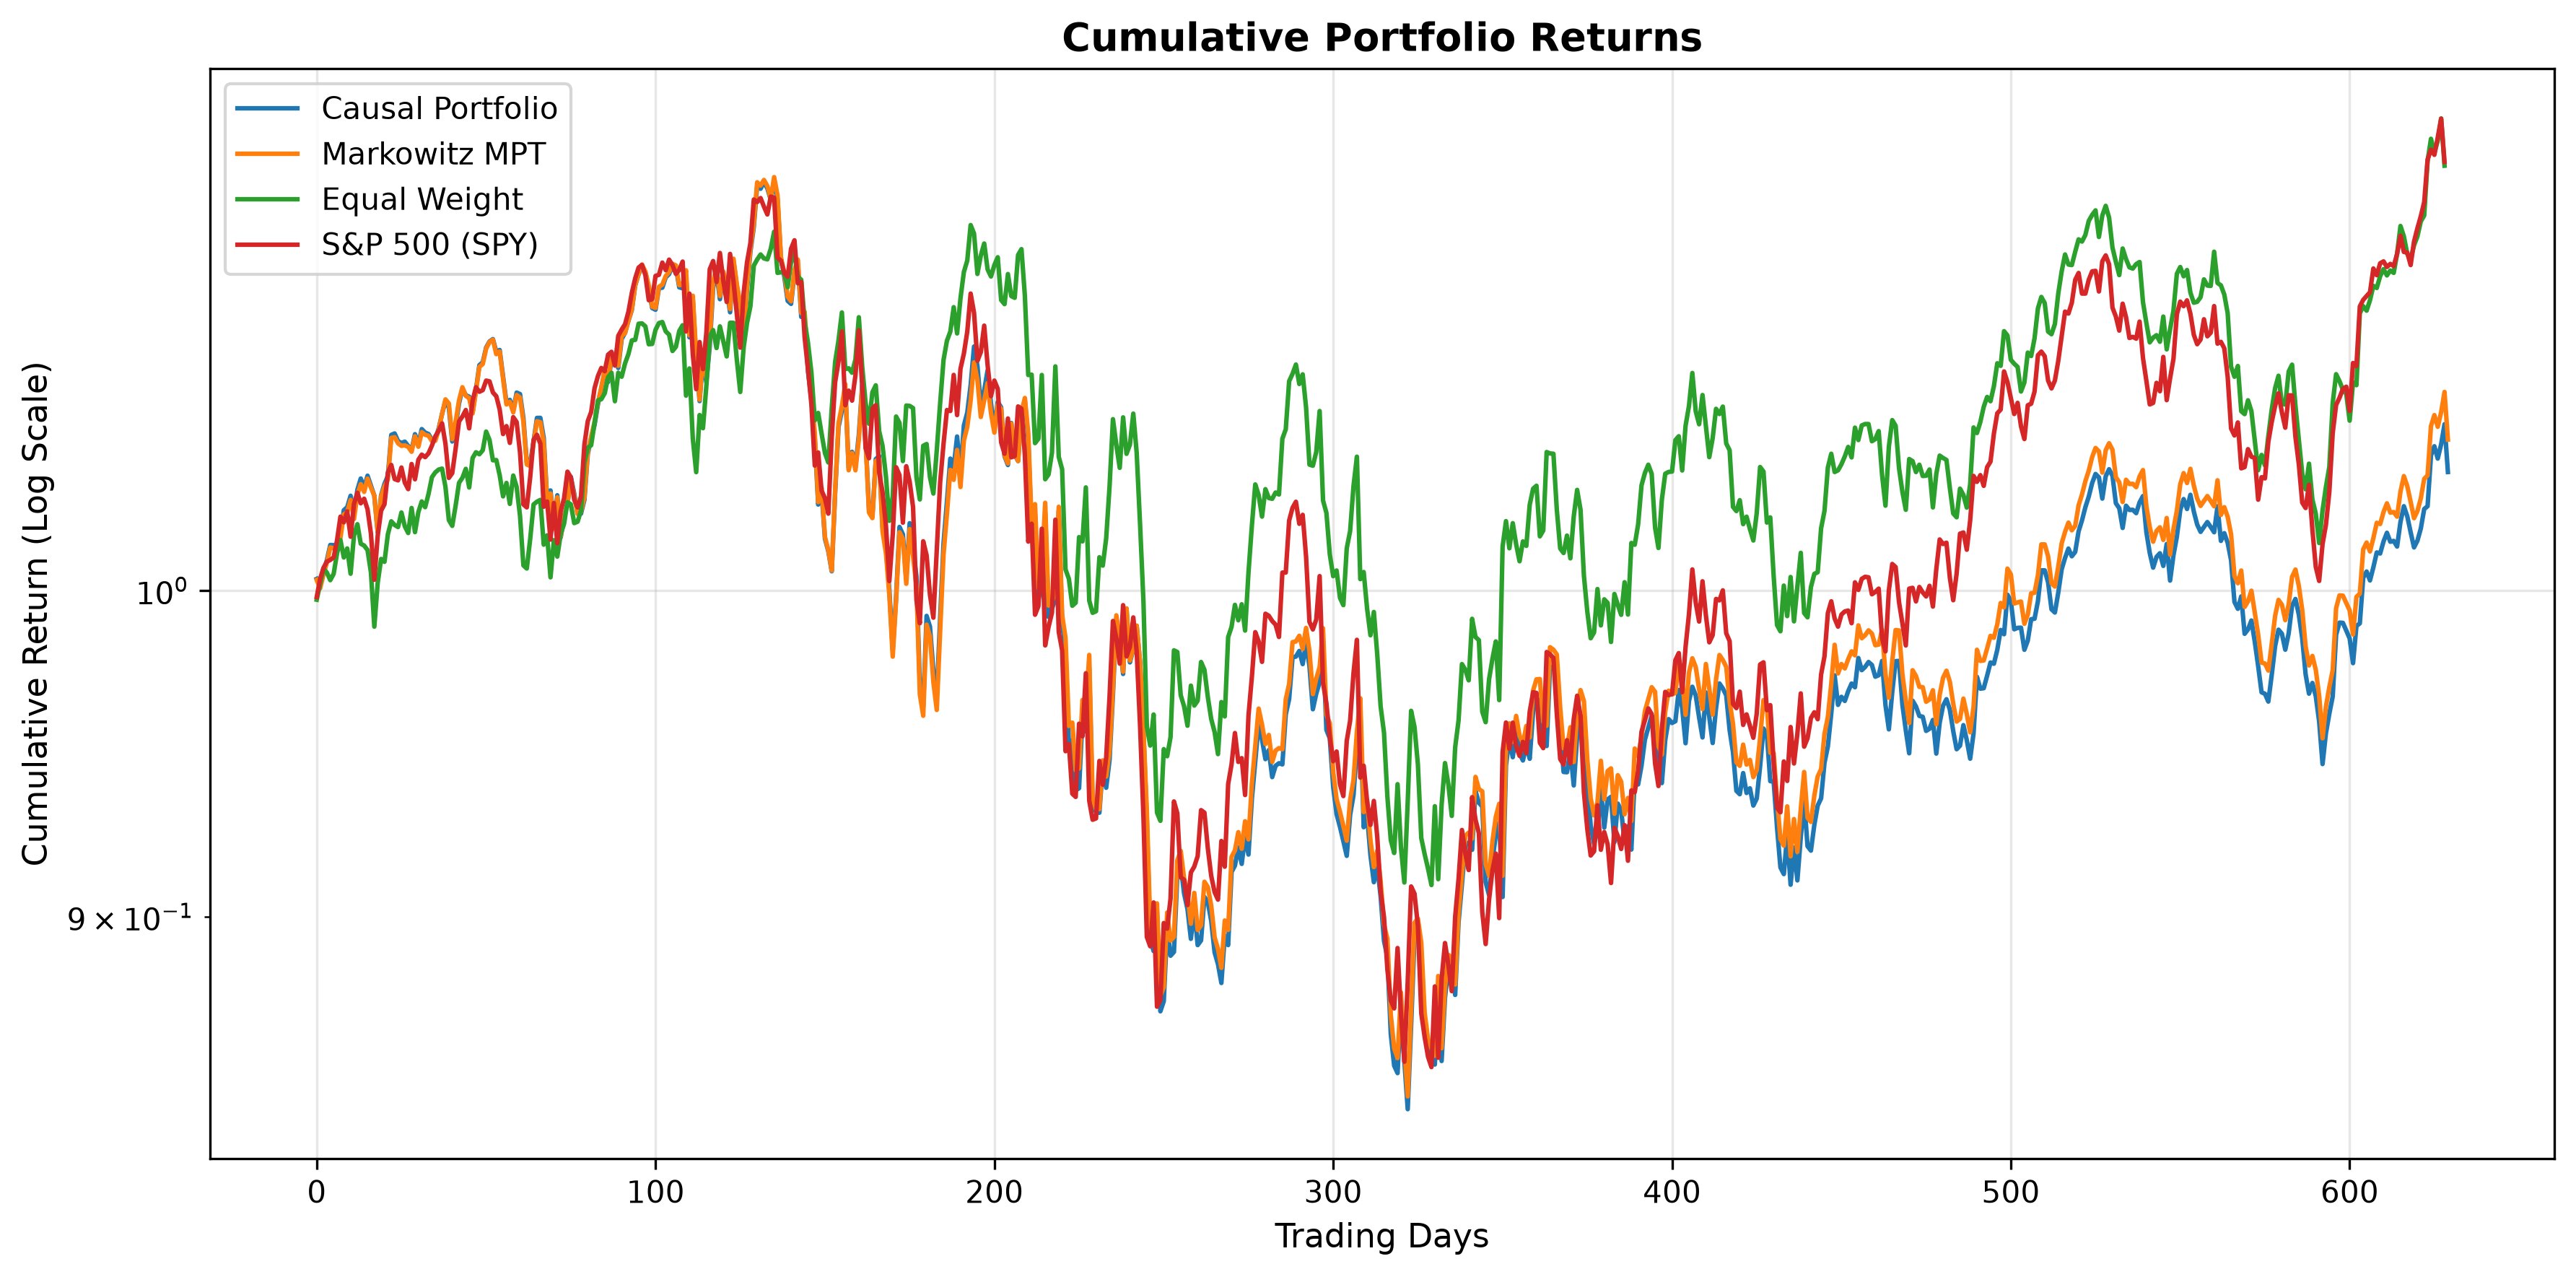
\includegraphics[width=\columnwidth]{figures/cumulative_returns.png}
\caption{Cumulative returns, walk-forward evaluation window.}
\label{fig:cumulative}
\end{figure}

\begin{figure}[h]
\centering
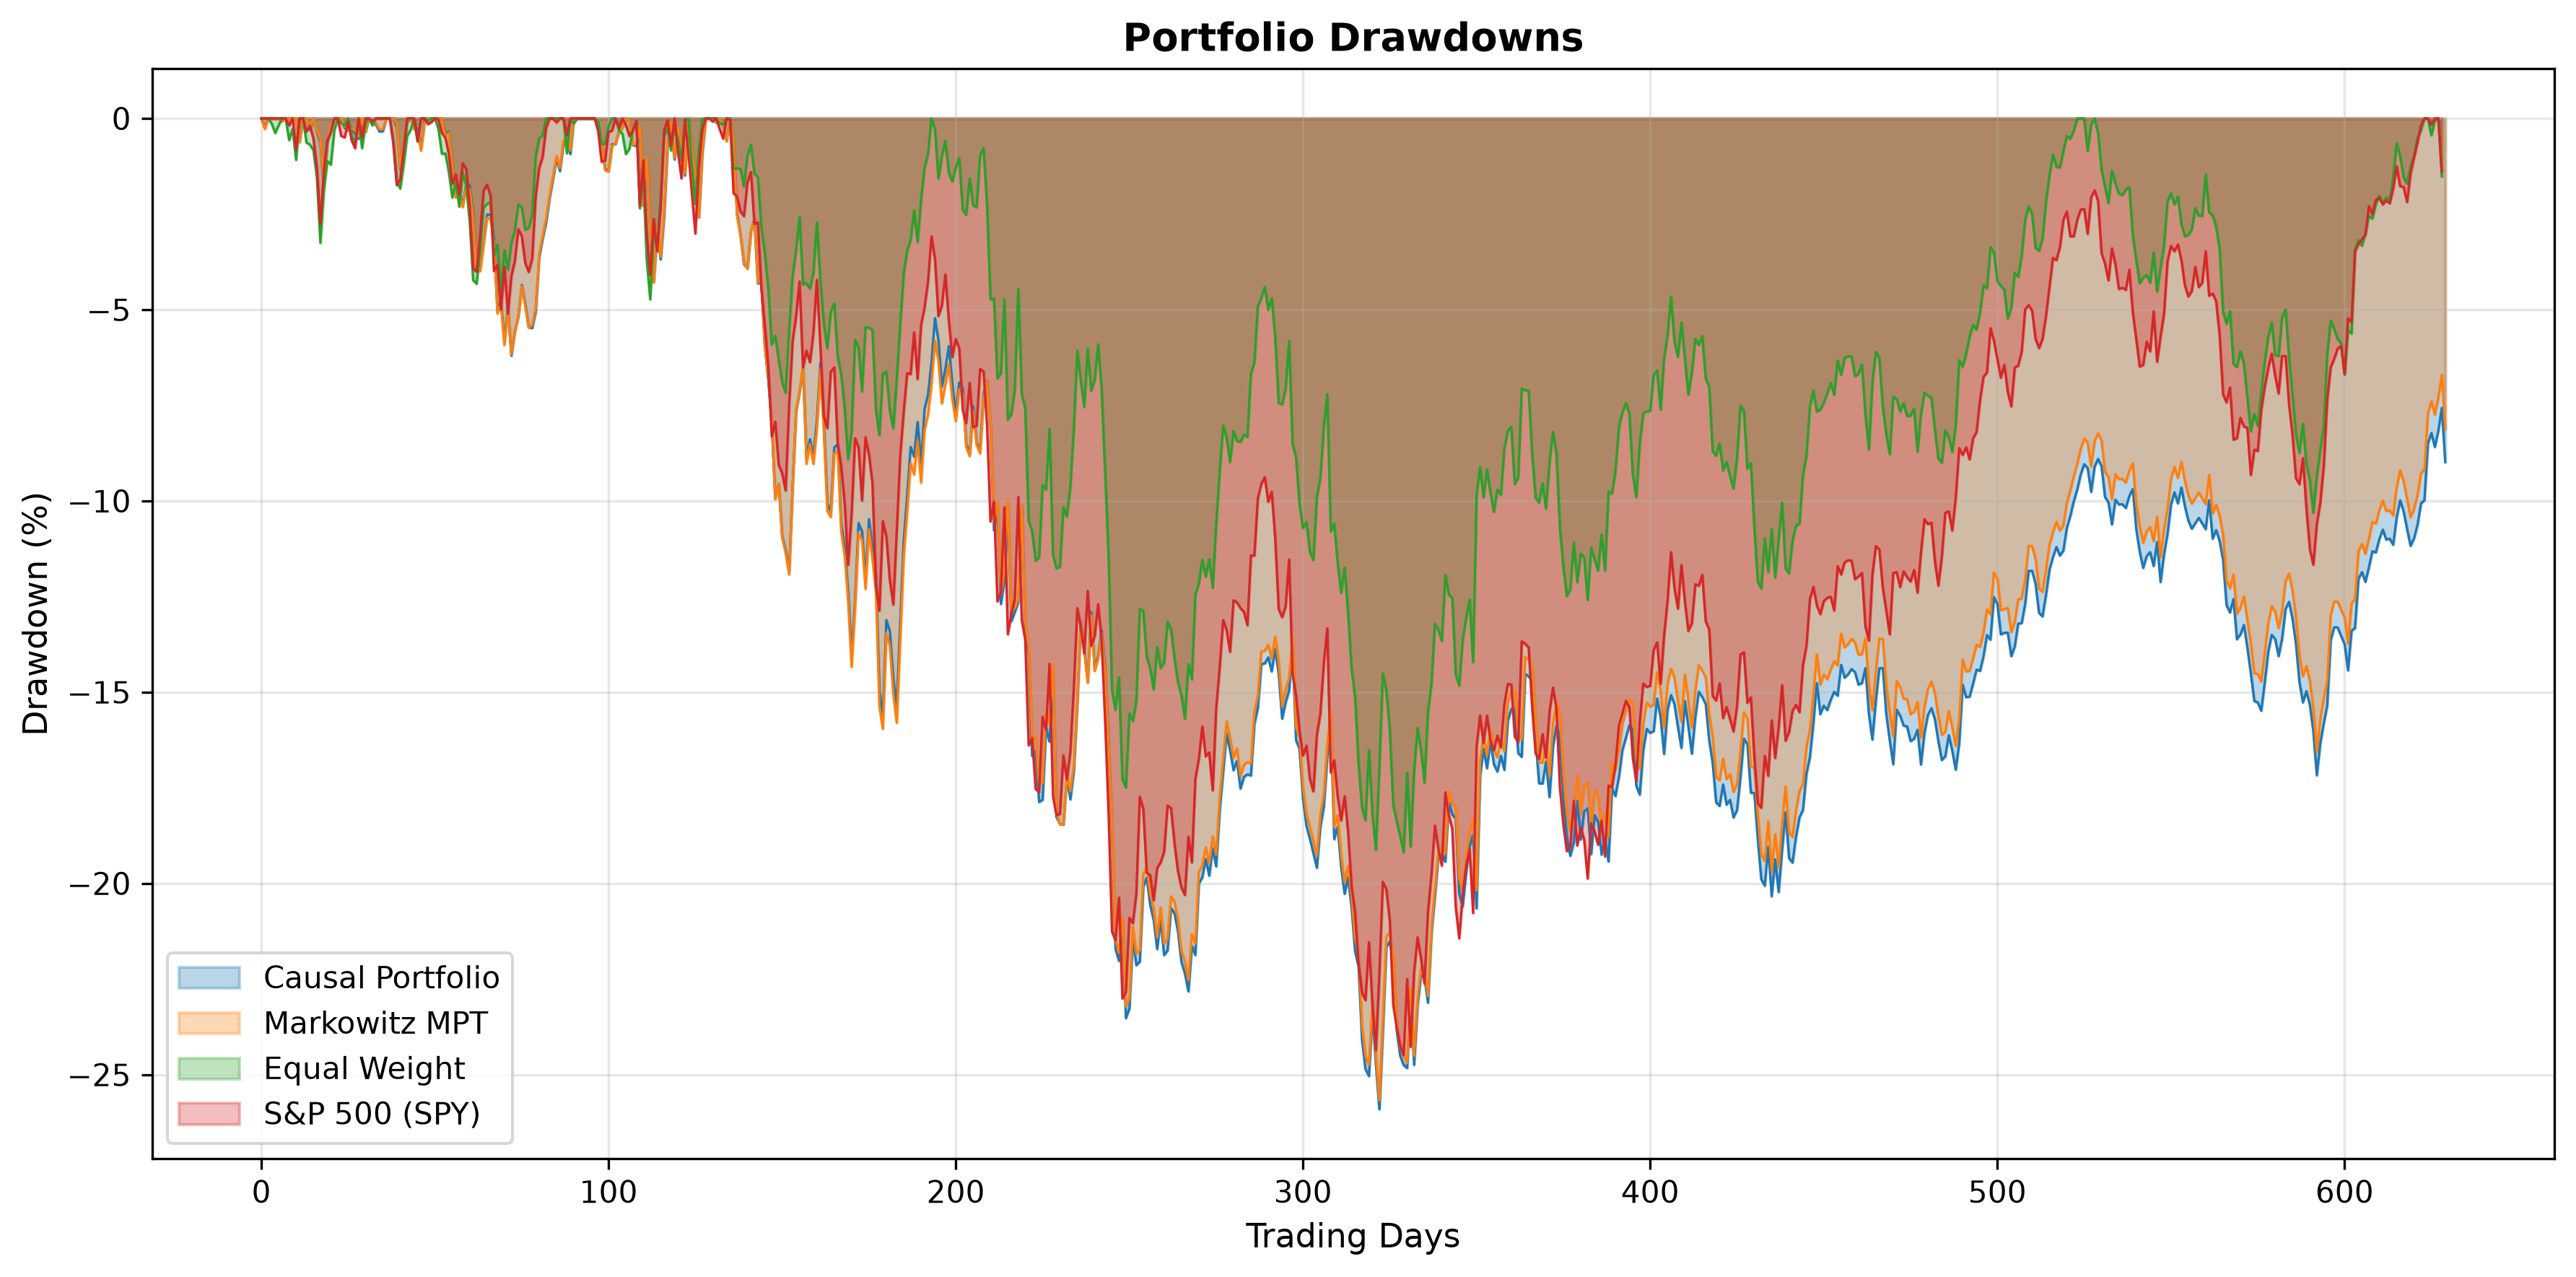
\includegraphics[width=\columnwidth]{figures/drawdowns.png}
\caption{Drawdown profile, walk-forward evaluation window.}
\label{fig:drawdown}
\end{figure}

\subsection{Statistical Significance}
Table \ref{tab:significance} reports paired $t$-tests, Mann--Whitney $U$
tests, and bootstrapped (10{,}000 resamples) 95\% confidence intervals for
the monthly Sharpe ratio of each strategy (source:
\texttt{results/phase4\_statistical\_significance.csv},
\texttt{phase4\_bootstrap\_sharpe.csv}).

\begin{table}[h]
\centering
\small
\caption{Significance tests, causal-blended vs.\ each baseline ($n=29$--$30$ monthly observations).}
\label{tab:significance}
\begin{tabular}{lrr}
\toprule
Comparison & Paired $t$ ($p$) & Mann--Whitney $U$ ($p$) \\
\midrule
vs.\ Equal Weight & $-0.94$ (0.356) & 442.0 (0.461) \\
vs.\ Markowitz MPT & $-1.13$ (0.267) & 442.5 (0.547) \\
vs.\ S\&P 500 & $-1.02$ (0.315) & 425.0 (0.563) \\
\bottomrule
\end{tabular}
\end{table}

No comparison is significant at conventional levels. Bootstrapped 95\%
Sharpe-ratio confidence intervals for all four strategies exceed 2.5
Sharpe units in width and cross zero (e.g., causal-blended: $[-1.30,
1.31]$), reflecting the limited statistical power of a $\sim$30-month
evaluation window for distinguishing Sharpe ratios --- a genuinely
high-variance statistic at this sample size, independent of which
strategy is under test. Figure \ref{fig:rolling-sharpe} shows the
rolling 12-month Sharpe ratio for all four strategies over the
evaluation window: the causal-blended and plain-Markowitz lines track
almost exactly on top of each other throughout, visually reinforcing
that the causal adjustment is a minor perturbation on the base
optimizer rather than a distinct source of return or risk.

\begin{figure}[h]
\centering
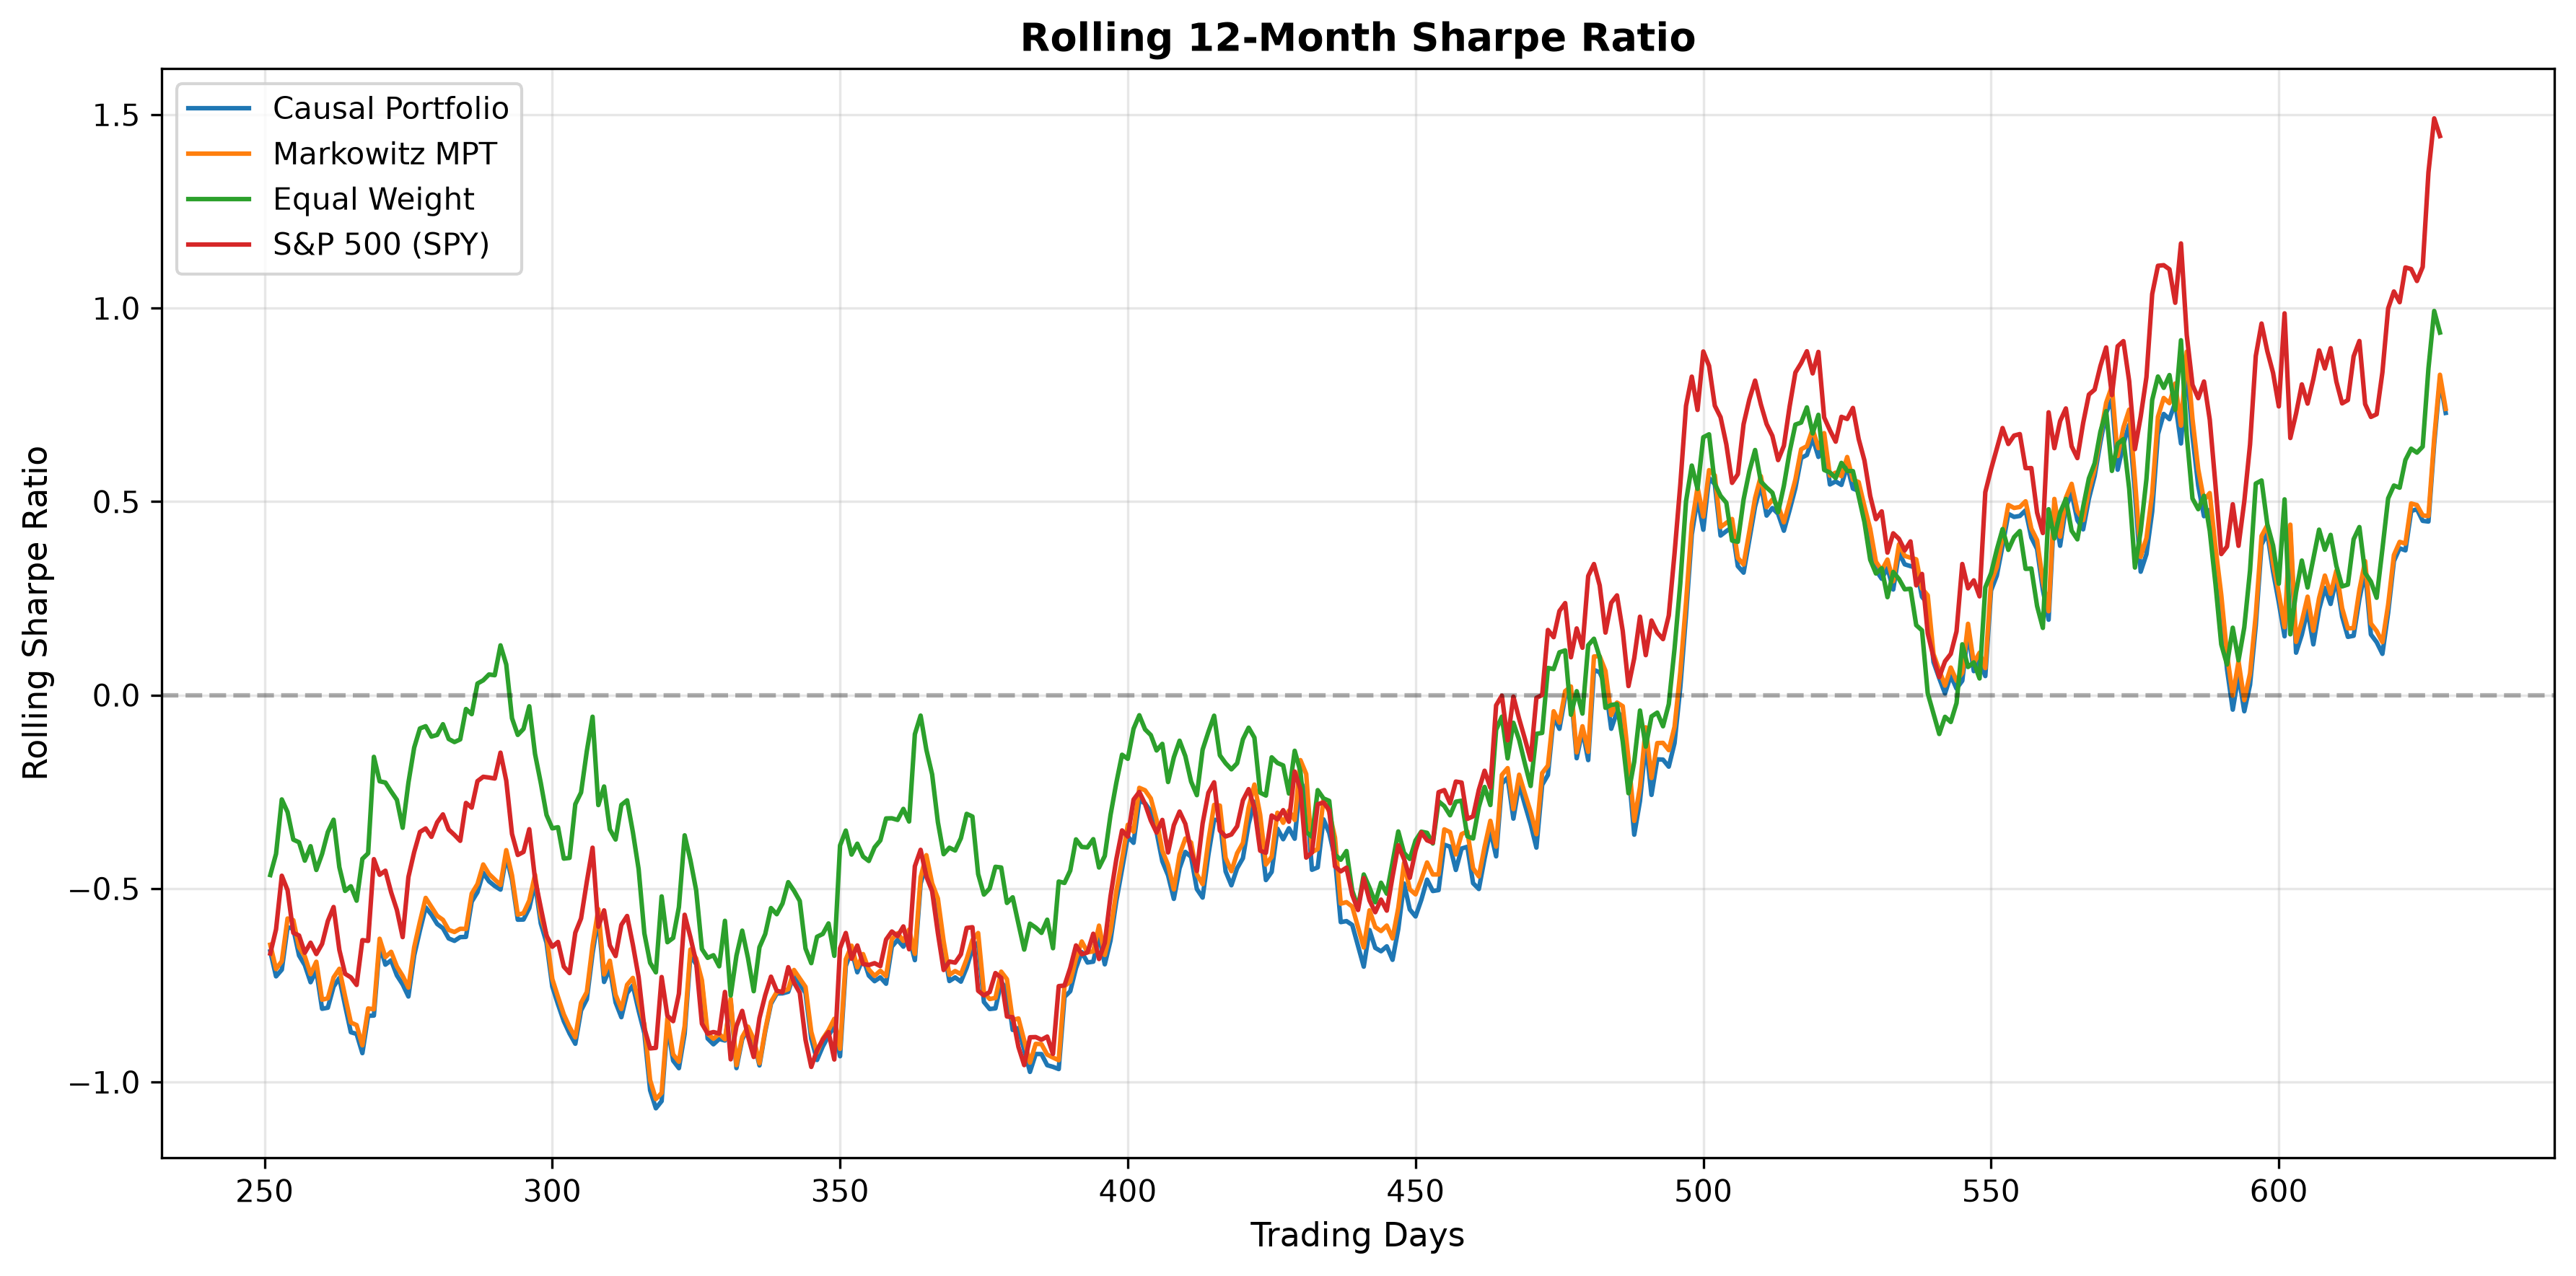
\includegraphics[width=\columnwidth]{figures/rolling_sharpe.png}
\caption{Rolling 12-month Sharpe ratio, walk-forward evaluation window.
The causal-blended and plain-Markowitz lines are nearly indistinguishable
throughout, consistent with the ablation result (Table
\ref{tab:ablation}) that the causal adjustment is a small perturbation
on the base optimizer.}
\label{fig:rolling-sharpe}
\end{figure}

\subsection{Ablation}
Table \ref{tab:ablation} isolates the contribution of specific causal
components by systematically removing or altering them (source:
\texttt{results/phase5\_ablation.csv}), all under the identical
look-ahead-corrected walk-forward protocol.

\begin{table}[h]
\centering
\small
\caption{Ablation study, $\Delta$Sharpe relative to the full causal model.}
\label{tab:ablation}
\begin{tabular}{lr}
\toprule
Variant & $\Delta$ Sharpe vs.\ full \\
\midrule
Full causal model & $0.000$ (Sharpe $-0.143$) \\
No causal graph (plain Markowitz) & $+0.024$ \\
No refutation validation & $0.000$ \\
No CATE (sector-uniform ATE) & $+0.025$ \\
Alt.\ treatment (VIX, not rates) & $+0.050$ \\
\bottomrule
\end{tabular}
\end{table}

Every ablation variant improves on, or matches, the full model; none
degrades it. This is the opposite of what an ablation study is
conventionally read to support: rather than showing each causal
component contributes positively, it shows the causal adjustment as
currently specified is a net negative in this sample, and that this
holds whether the adjustment is removed entirely, made cruder (uniform
rather than heterogeneous), or redirected to a different primary
treatment variable.

\subsection{Robustness}
Table \ref{tab:robustness} summarizes four robustness checks (source:
\texttt{results/phase6\_*.csv}), all re-run under the corrected
methodology.

\begin{table}[h]
\centering
\small
\caption{Robustness checks (Sharpe ratio).}
\label{tab:robustness}
\begin{tabular}{lr}
\toprule
Check & Sharpe \\
\midrule
Full 11-sector universe & $-0.143$ \\
Large-cap 5-sector universe & $-0.225$ \\
Transaction cost: 0 bps & $-0.138$ \\
Transaction cost: 50 bps & $-0.164$ \\
Split shifted $-6$mo (test starts 2020-11) & $-0.143$\textsuperscript{a} \\
Split shifted $+6$mo (test starts 2021-11) & $-0.408$ \\
\bottomrule
\end{tabular}
\end{table}
\vspace{-0.5em}
\noindent{\footnotesize\textsuperscript{a}Coincides with the baseline
fold sequence: both requested start dates fall within the effective data
history's first 756 days for the full universe, so the walk-forward
anchor clamps to the same realized fold sequence. Not an independent
check for this universe/window-length combination.}

Reducing transaction costs to zero still leaves Sharpe negative
($-0.138$), indicating that costs are not the primary driver of
underperformance. The $+6$-month split is substantially worse
($-0.408$), driven by the removal of two strongly positive early folds
(Section \ref{sec:limitations}) rather than a systematic split-date
effect. Two named sub-periods (Pre-COVID: 2018-01-01 to 2019-12-31;
COVID Crash: 2020-01-01 to 2020-12-31) could not be evaluated: the
youngest constituent ETF in the 11-sector universe (XLC) only began
trading 2018-06-19, leaving insufficient history before these windows to
support even one 756-day training fold.

As a secondary, clearly-labeled robustness check, we also evaluate a
window (2023-03-08 to 2024-01-01) that is leak-free even under the
original, uncorrected global model, since it falls entirely after that
model's training cutoff. Over this short window (3 realized folds), the
causal-blended portfolio narrowly outperforms plain Markowitz (Sharpe
$+0.688$ vs.\ $+0.667$). We report this for completeness but do not treat
it as informative: three quarterly folds provide essentially no
statistical power, and it should not be read as contradicting the
primary result.

\subsection{Multiple-Comparisons Correction}
Of all 77 macro-sector treatment-effect pairs evaluated (7 treatments
$\times$ 11 sectors; \texttt{results/phase2\_ate\_results.csv}), 27 are
significant at an uncorrected $\alpha=0.05$. Applying
Benjamini--Hochberg false-discovery-rate correction
\citep{benjamini1995controlling} leaves 18 significant pairs. We report
both counts throughout rather than the uncorrected count alone. Unlike
the portfolio-level result in Section \ref{sec:results}, this is not a
null finding: nearly a quarter of the tested treatment-effect pairs are
statistically robust to multiple-comparisons correction, concentrated in
rate-sensitive and defensive sectors (Utilities, Real Estate,
Financials) responding to Fed Funds Rate, GDP, Unemployment, and VIX
changes. Section \ref{sec:limitations} discusses why effects this real
still fail to move the blended portfolio's realized performance.

This 5$\times$5-vs-7$\times$11 restriction was specific to the standalone
evaluation script that produces this subsection's numbers; we separately
verified that the per-fold treatment-effect refit driving the headline
walk-forward backtest (Section \ref{sec:leakage-fix}) and the live-serving
model both already iterate the full 7-treatment, 11-sector grid, so the
headline results in Section \ref{sec:results} were not affected by this
bug and did not need to be re-run.

\section{Limitations and Threats to Validity}
\label{sec:limitations}

\textbf{Identification assumptions.} Every treatment-outcome pair uses
the same two-variable confounder set (S\&P 500 return and its 21-day
volatility). This is a minimal backdoor-adjustment specification. It
does not rule out reverse causality between sector returns and the
macro treatments themselves: the Federal Reserve's rate-setting reaction
function is explicitly forward-looking and responds to market and
inflation expectations, so part of an estimated ``effect'' of a rate
change on sector returns could reflect the Fed reacting to information
that also independently moved returns, not returns responding to the
rate change. Our causal graph specification assumes the treatment-to-outcome
direction and does not test for or adjust against this.

\textbf{Sample size.} The evaluation window yields 10 walk-forward folds
and $\sim$30 monthly return observations for parametric and
nonparametric significance testing --- sufficient to report point
estimates but not to detect anything but a large effect with
statistical confidence, as reflected in the width of the bootstrapped
Sharpe confidence intervals.

\textbf{Effect magnitude relative to estimation error.} A supplementary
fold-level analysis of the base optimizer
(\texttt{backend/scripts/diagnose\_fold\_concentration.py}, output saved to
\texttt{results/fold\_concentration\_diagnostic.csv}) shows the
walk-forward Markowitz layer concentrating up to its 20\% per-asset cap in
whichever 1--2 sectors had the best trailing 3-year return, while
assigning zero weight to the sector with the highest trailing volatility
-- a textbook illustration of mean-variance optimization's sensitivity to
estimation error rather than a causal-signal failure. During one fold
(test window March--June 2022), this concentration coincided with a broad
growth-sector selloff that the zero-weighted, high-trailing-volatility
sector (Energy) did not participate in, producing an approximately
$-42\%$ single-quarter portfolio return. The causal adjustment's
magnitude in this diagnostic (typically 0.1--1.7 percentage points on
expected returns already dispersed 11--37\% across sectors in the
affected folds) is too small, by roughly one to two orders of magnitude,
to materially redirect this concentration. This explains why the causal
signal is neither a strong positive nor a strong negative in aggregate:
it is largely a minor perturbation on a base optimization process whose
own behavior dominates the result.

\textbf{Data history constraint.} The youngest constituent of the
11-sector universe (XLC) began trading in mid-2018, which is why two
named historical sub-periods could not be evaluated under the
756-day walk-forward protocol, and why the $-6$-month split-sensitivity
check did not produce an independent fold sequence from the baseline.

\textbf{Reproducibility of the corrected result.} All numbers in Section
\ref{sec:results} were produced by re-running the evaluation scripts
against the corrected code and are reproducible from the repository;
we do not report numbers that could not be traced to a specific script
output.

\section{Conclusion}

We built and evaluated a system combining causal discovery, double
machine learning treatment-effect estimation, regime detection, an ML
forecasting ensemble, and a causally-blended portfolio optimizer. In the
process of evaluating it rigorously, we found and corrected a
look-ahead bias in our own treatment-effect model's training protocol,
and found that this correction reverses the paper's central empirical
comparison: the causal adjustment does not improve on plain Markowitz
optimization once evaluated point-in-time, and neither optimized
strategy significantly outperforms a passive benchmark or naive
diversification in this sample. We consider the corrected evaluation
protocol --- refitting the causal component per walk-forward fold, not
only the portfolio-optimization layer --- to be reusable independent of
this paper's specific negative result, and we report the negative
result itself as evidence about the practical difficulty of extracting
a usable tactical allocation signal from causal treatment-effect
estimates at this data scale, rather than omit it.

\bibliographystyle{plainnat}
\bibliography{references}

\end{document}
